
\title{Recap System and device programming (01NYHOV)}
\author{Jacopo Nasi\\
        Computer Engineer\\
        Politecnico di Torino}
\date{II Period - 2017/2018\\\bigskip\bigskip\today}

\documentclass[12pt]{article}
\usepackage[utf8]{inputenc}
\usepackage[italian]{babel}
\usepackage{geometry}
\usepackage{indentfirst} % First line indent
\usepackage{mathtools}
\usepackage{wrapfig}
\usepackage[usenames, dvipsnames]{color}
\usepackage{float}
\usepackage{amssymb}
\usepackage{ifsym}
% Misure Documento
\geometry{ a4paper, total={170mm,257mm},left=35mm, right=35mm, top=35mm, bottom=35mm }

\begin{document}

\begin{figure}
  \centering
  
\includegraphics[width=10cm]{images/polito.pdf}
\end{figure}

\maketitle

\newpage
\tableofcontents

\newpage
{\noindent \Large \textbf{License}\bigskip}

This work is licensed under a Creative Commons Attribution-NonCommercial-ShareAlike 3.0 Unported License.\\
You are free:
\begin{itemize}
  \item \textbf{to Share}: to copy, distribute and transmit the work
  \item \textbf{to Remix}: to adapt the work
\end{itemize}
Under the following conditions:
\begin{itemize}
  \item \textbf{Attribution}: you must attribute the work in the manner specified by the author or licensor (but not in any way that suggests that they endorse you or your use of the work)
  \item \textbf{Noncommercial}: you may not use this work for commercial purposes.
  \item \textbf{Share Alike}: if you alter, transform, or build upon this work, you may distribute the resulting work only under the same or similar license to this one.
\end{itemize}

\noindent More information on the Creative Commons website (http://creativecommons.org).

\begin{figure}[h!]
  \centering
  
\includegraphics[width=3cm]{images/license.png}
\end{figure}

{\noindent \Large \textbf{Acknowledgments}\bigskip}

Questo breve riepilogo non ha alcuno scopo se non quello di agevolare lo studio di me stesso, se vi fosse di aiuto siete liberi di usarlo.\\
Le fonti su cui mi sono basato sono quelle relative al corso offerto (\textbf{System and device programming (01NYHOV)}) dal Politecnico di Torino durante l'anno accademico 2017/2018.\\
Non mi assumo nessuna responsabilità in merito ad errori o qualsiasi altra cosa. Fatene buon uso!
\newpage


\section{Review}
\subsection{Processes}
An \textbf{Algorithm} is a logical procedure that in a finite number of steps solves problem. A \textbf{Program} is a formal expression of an algorithm by means of a programming language. The \textbf{Process} is a sequence of operations performed by a program in execution on a given set of input data. The structure of a process, figure \ref{fig:proc_mem} is made by:
\begin{itemize}
  \item Text area (source code)
  \item Data Area (global variables)
  \item Stack (functions parameters and local variables)
  \item Heap (dynamic variables allocated during the process execution)
  \item Registers (program counter, stack pointer, ecc...)
\end{itemize}
\begin{figure}[H]
  \centering
  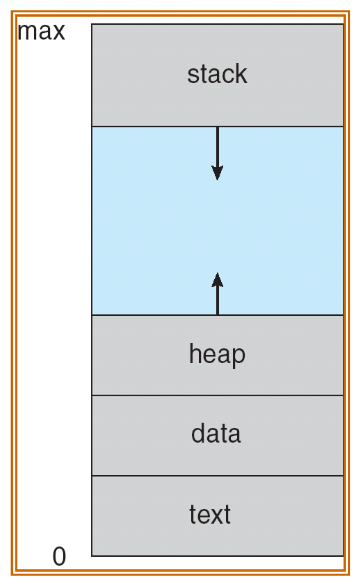
\includegraphics[width=0.5\linewidth]{images/proc_mem.png}
  \caption{Process memory layout}
  \label{fig:proc_mem}
\end{figure}
The trace of a process is its entire line, it represent the state at any time. An important operation is the possibility to freeze the state of a process in order to execute other tasks. This choice is demanded to the CPU scheduler. The possibility to switch from a state sto another is called \textbf{Context Switching}.\\
Each processes has a unique (while the process is active) identifier (\textbf{PID}), a positive integer.\\
The \textbf{\textit{fork()}} is the system call used to create a new child process. The child is a copy of the parent execluding the Processs ID returned by the fork.
\begin{itemize}
  \item The parent process receives the child PIDs.
  \item The child process receives the value 0.
\end{itemize}
The 2 processes are perfect clones with 2 different heap, 2 stacks, etc... The only shared part is the code. A process can become orphan if the parent dies, in that case is become son of the INIT process (PID: 1). Another possible state is the zombie, where the process has terminated its execution but still has an entry in the process state. The zombie state waste resources and must be avoided. During the fork process the child inherit the value of local variable from the parent but they are different varible and they aren't linked, the address space of the 2 processes is different.
There are several way to exit from a process:
\begin{itemize}
  \item \textit{return}
  \item \textit{exit}
\end{itemize}
there are also other not correct termination, like \textit{abort}. The correct behaviour require that the parent \textbf{\textit{wait()}} for the process terminations of tis sons, the kernel sends a signal (\textbf{SIDCHLD}) to its parent. The parent can manage or ignore it.\\
The system call \textbf{\textit{exec()}} is different from the fork because it run a different executable, it does not create another process, it substitutes the calling process image with the image of another program.

\subsection{Operating System}
The OS is not a program, is a set of modules, a big interrupt routine. It reacts to action like mouse moving, ecc... The user can't exxecute all the instriction set. The CPU runs in at least 2 states (mode):
\begin{itemize}
  \item Kernel
  \item User
\end{itemize}
Each mode defined different access rights, of course the kernel mode is the most powerfull. The are some instruction that are priviledged, like the I\/O, or over some registers due to concurrency where the controll is CPU demanded.\\
\subsection{Kernel}
The kernel is a black box, the only way to interact with it is to used the interrupts provided. By receiving and address the kernel know that it must perform, for example, a reading operation and so on. Is not possible to access directly to the kernel memory.

\subsection{Shell}
The shell is not part of the kernel, is like all other processes. The user perform, through it, system calls that run at the user level.

\subsection{Threads}
The process are really "exprensive" in case of cooperation, the clone operation involves a significant increase of memory used and the creation time become an overhead. Also the context switching can become expensive. A possible solution to all these problem is using \textbf{threads}. For the kernel different threads are part os a single process. The context switch is really faster because the context "is the same". The process is the owner of the resources that are used by all its threads. The thread is the basic unit of CPU utilization (and scheduling). They are also called lightweight processes.
\begin{figure}[H]
  \centering
  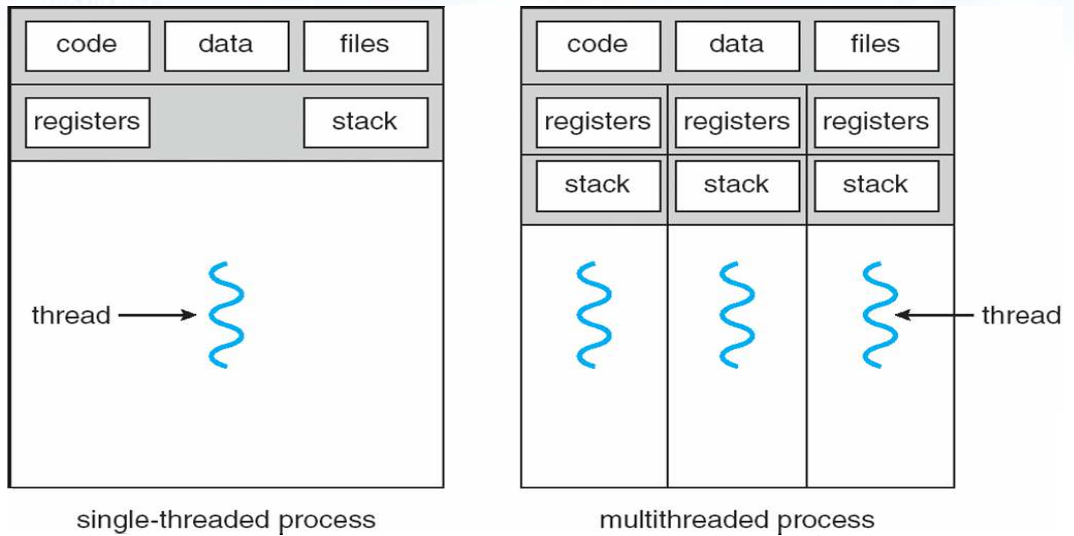
\includegraphics[width=0.5\linewidth]{images/proc_thread.png}
  \caption{Processes and Threads}
  \label{fig:proc_thread}
\end{figure}

\subsection{Critical section}
Also know as Critical Region, is a section of code, common to multiple threads, in which they can access (read and write) shared objects. A section in which threads are competing for the use (R\/W) of shared resources. We want to ensure that when one thread is executing in its CS, no other thread is allowed to execute in its CS. THe solution is to establish an access protocol to enter the critical section in \textbf{mutual exclusion}.\\
There are different solutions to solve this problem:
\begin{itemize}
  \item software
  \item hardware
  \item System Call (semaphore)
\end{itemize}

\subsection{Semaphore}
System call used to manage critical sections and to solve synchronization problem. The semaphore primitives allows thread to:
\begin{itemize}
  \item Create semaphore (init)
  \item Be blocked on the semaphore (wait)
  \item Wakeup if it was blocked (signal)
  \item Destroy a sempahore (destroy)
\end{itemize}
The operations on a semaphore are \textbf{ATOMIC}, it is impossible for two threads to perform simultaneously operations on the same semaphore.\\
Another type of semaphore is the MUTEX, or binary semaphore, they are a little bit easier to be managed but they are less powerfull. Only the action lock and unlock must be performed.\\
Sempahores can be also implemented like pipes.

\section{Memory Management}
Chapter about hardware memory organization, discussing MM techniques like paging and segementation.

\subsection{Background}
A program must be brought (from disk) into main memory and placed within a process for it to be run. Main memory and registers are onyl CPU storage and only it can access directly to them. The register access is performed in one CPU clock, the main memory could require more cycles, the cache instead is between them (speed speaking).\\
The address binding of instructions and data to memory addresses can happen at three different stages:
\begin{itemize}
  \item \textbf{Compile Time}: If memory location know a priori, absolute code can be generated; must recompile code if starting location changes.
  \item \textbf{Load Time}: Must generate relocatable code if memory location is not know at compile time.
  \item \textbf{Execution Time}: Binding delayed until run time if the process can be moved during its execution from one memory segment to another. Need hardware support for address maps. (e.g. base and limit register)
\end{itemize}
\begin{figure}[H]
  \centering
  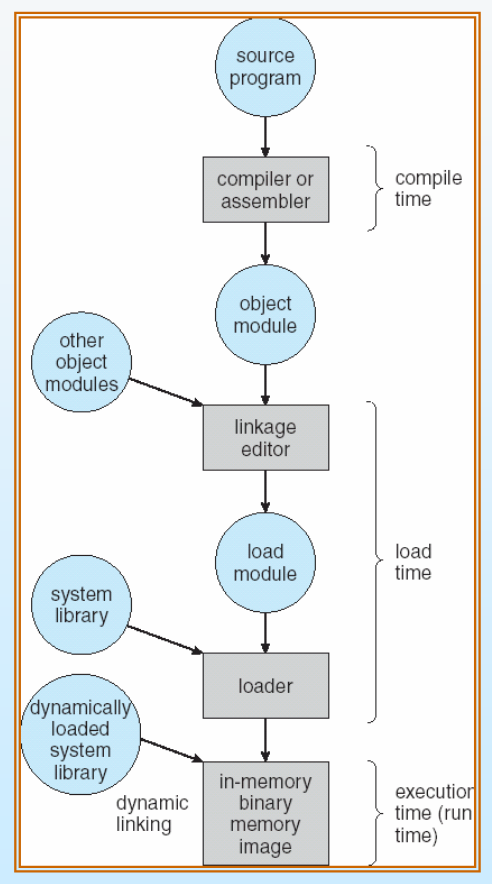
\includegraphics[width=0.4\linewidth]{images/multi_step_user.png}
  \caption{Multistep processing of a user program}
  \label{fig:multi_step_user}
\end{figure}

The concept of a logical addresses space that is bound to a separta physical address space is central to proper memory management.
\begin{itemize}
  \item \textbf{Logical}: Generated by the CPU; also referred as \textbf{virtual addresses}.
  \item \textbf{Physical}: Address seen by the memory unit.
\end{itemize}
Logical and physical addresses are the same in compile-time and load-time address-binding schemes; logical (virtual) and physical addresses differ in execution-time address-binding scheme.\\
The \textbf{MMU} (\textit{Memory-Management Unit}) is an hardware device that maps virtual to physical address. In its scheme, the value in the relocation register is added to every address generated by a user process at the time it is sent to memory. Every user program deals only with logical addresses.\\
Using the \textbf{Dynamic Loading} routine is not loaded until it is called, this allows a better memory space utilization (unused routine is never loaded). This function is useful when large amounts of code are needed to handle infrequently occuring cases.\\
Another important mechanism is the \textbf{Dynamic Linking} where the linking is postponed until execution time. Small piece of code, \textit{stub}, used to locate the appropriate memory-resident library routine, replaces itself with the address of the routine, and executes the routine. OS needed to check if routine is in processes memory addresses. This solution is particularly useful for libraries. It is also know as \textbf{Shared Libraries}.

\subsection{Swapping}


















\end{document}
